\documentclass[12pt,letterpaper]{article}
\usepackage[bottom=1in, top=1in, left=1in, right=1in]{geometry}
\usepackage[intlimits]{amsmath}
\usepackage{mathtools} % for splitfrac
\usepackage[utf8]{inputenc}
\DeclareUnicodeCharacter{2212}{-}
\usepackage{amsfonts,amssymb}
\DeclareSymbolFontAlphabet{\mathbb}{AMSb}
\usepackage{slashed}
\usepackage{textcomp}

\usepackage{float}
\usepackage[]{caption,subcaption}
\setcaptionmargin{0.5in}

\usepackage{fancyhdr}
%\usepackage{fancyheadings} % what does this do?
\usepackage{fancybox}

\usepackage{ifthen}
\usepackage{lscape,afterpage}
\usepackage{xspace}

\usepackage{siunitx}
\sisetup{detect-weight=true, detect-family=true}

\usepackage{xcolor}

\usepackage{appendix}

\usepackage{enumitem}

% table packages and commands
\usepackage{tabularx,booktabs}
\usepackage{dcolumn}
\usepackage{multirow}

\usepackage{longtable}

\usepackage{pdflscape}
\usepackage{afterpage} % can maybe be used to deal with text around landscape tables if I have troubles down the line
\usepackage{rotating}

% https://tex.stackexchange.com/questions/13509/biblatex-in-a-nutshell-for-beginners
% if I get the error, ".bbl not created by bib latex", run biber $, where $ is the basename of the main .tex file, then rerun the build
\usepackage[sorting=none]{biblatex}
\addbibresource{myBib.bib}
% \addbibresource(othersfiles.bib) % if I ever split up the bibiliography add multiple resources like this

%feynman digram package
% \usepackage{tikz-feynman} % doesn't work out of the gate, wants LuaLaTex - see https://jpellis.me/projects/tikz-feynman/
% \tikzfeynmanset{compat=1.1.0} 
\usepackage[compat=1.1.0]{tikz-feynhand} % simpler version of tikz-feynman - see https://ctan.org/pkg/tikz-feynhand?lang=en

%==========================================================================%
%%% graphicx and pdf creation
\usepackage{graphicx}

\usepackage{hyperref} % set up this package last (or almost last anyways)
% \hypersetup{
%     colorlinks,
%     linkcolor={red!50!black},
%     citecolor={blue!50!black},
%     urlcolor={blue!80!black}
% }

% \usepackage{glossaries} % might be able to use this to make an alphabetically ordered list of abbreviations - needs to be set up after hyperref

\interfootnotelinepenalty=10000 % hack to force footnotes to one page

%==========================================================================%
%               USEFUL MACROS AND COMMANDS
%==========================================================================%

\newcommand{\figref}[1]{Figure~\ref{#1}}
\newcommand{\chapref}[1]{Chapter~\ref{#1}}
\newcommand{\secref}[1]{Section~\ref{#1}}
\newcommand{\appref}[1]{Appendix~\ref{#1}}
\newcommand{\refref}[1]{Reference~\cite{#1}}
\newcommand{\equref}[1]{Equation~\ref{#1}}
\newcommand{\tabref}[1]{Table~\ref{#1}}

\newcommand{\latex}{\LaTeX\xspace}
\newcommand{\ROOT}{\texttt{ROOT}\xspace}


\def\BU{BOSTON UNIVERSITY}
\def\Bu{Boston University}
\def\GSA{GRADUATE SCHOOL OF ARTS AND SCIENCES}
\def\Gsa{Graduate School of Arts and Sciences}

\def\wa{$\omega_{a}$\xspace}
\def\chisq{$\chi^{2}$\xspace}
\def\gmtwo{$g-2$\xspace}
\def\Ta{$T_{a}$\xspace}
\def\Tatwo{$T_{a}/2$\xspace}
\def\amu{$a_{\mu}$\xspace}
\def\g{$g$\xspace}

\def\mutau{\SI{2.2}{\micro s}\xspace}
\def\taumu{$\tau_{\mu}$\xspace}

\newcommand{\ns}[1]{\SI{#1}{ns}\xspace}
\newcommand{\mus}[1]{\SI{#1}{\micro s}\xspace}
\newcommand{\mum}[1]{\SI{#1}{\micro m}\xspace}

\newcommand{\ppb}[1]{\SI{#1}{ppb}\xspace}


\def\eV{\text{e\kern-0.15ex V}\xspace}
\def\keV{\text{k\eV}\xspace}
\def\MeV{\text{M\eV}\xspace}
\def\GeV{\text{G\eV}\xspace}
\def\TeV{\text{T\kern-0.1ex \eV}\xspace}

\def\DT{$\Delta t_{12}$\xspace}

\def\R{$R$\xspace}
\def\dR{$\delta R$\xspace}
\def\DR{$\Delta R$\xspace}
\def\K{$\kappa_{loss}$\xspace}

\def\RE{ReconEast\xspace}
\def\RW{ReconWest\xspace}

\def\Rone{Run~1\xspace}

\newcolumntype{L}{D{.}{.}{2,3}} % define a column type L with specific spacing before and after the decimal point
\makeatletter
\newcolumntype{B}{>{\boldmath\DC@{.}{.}{2,3}}l<{\DC@end}} % define a column that's bold and does the above
\makeatother

\newcolumntype{F}{D{.}{.}{3,1}}
\newcolumntype{E}{D{.}{.}{3,3}}

\newcolumntype{Z}{D{.}{.}{1,4}}
% \newcolumntype{Z}{D{.}{.}{1,4}>{\centering}p{2em}}

\newcolumntype{H}{D{.}{.}{1,1}}
\makeatletter
\newcolumntype{J}{>{\boldmath\DC@{.}{.}{1,1}}l<{\DC@end}} % define a column that's bold and does the above
\makeatother

\newcolumntype{G}{D{.}{.}{2,1}}
\makeatletter
\newcolumntype{K}{>{\boldmath\DC@{.}{.}{2,1}}c<{\DC@end}} % define a column that's bold and does the above
\makeatother

\newcolumntype{O}{>{\centering\arraybackslash}X}

% \makeatletter
% \newcolumntype{Y}{>{\DC@{.}{.}{2,1}}X<{\DC@end}}
% \makeatother

\newcolumntype{Y}{D..{3.1}}

% \newcolumntype{Y}{>{\centering\arraybackslash}D{.}{.}{2,1}}


\usepackage{array}
% \newcolumntype{R}[1]{>{\centering\arraybackslash}p{#1}} % for wrapping text
\newcolumntype{R}[1]{>{\raggedright\let\newline\\\arraybackslash\hspace{0pt}}m{#1}}

% command to make row in table bold
\newcommand\setrow[1]{\gdef\rowmac{#1}#1\ignorespaces}
\newcommand\clearrow{\global\let\rowmac\relax}

\newcommand*{\thead}[1]{\multicolumn{1}{c}{#1}} % define a new command thead which centers table headers in the first row and works with the rest of the table environment



%==========================================================================%
% BEGIN
%==========================================================================%

\title{Statistical Correlations Between \R1 \wa Analyses}
\author{Nicholas Kinnaird}
\date{\today}

\begin{document}

\maketitle

\begin{abstract}
	This note describes the implementation and use of a Monte Carlo simulation taking real data input in order to determine statistical correlations between the different \Rone $\omega_{a}$ analyses. These statistical correlations are needed in order to properly combine the results. These statistical correlations include the effects from the different reconstructions, different analysis methods (TARQ), and different analyzer analysis parameters. The statistical correlations here can be used as a starting point going forward for combinations of future \wa analyes. This note does not describe the combination methodology proposed, which will be detailed in a separate note.
\end{abstract}


% The content of the thesis
%!TEX root = ../StatisticalCorrelations.tex

\graphicspath{{Body/Figures/}}

\clearpage
\section{Introduction}

%!TEX root = ../StatisticalCorrelations.tex

\graphicspath{{Body/Figures/}}

\clearpage
\section{Monte Carlo}

% \input{Body/FitVerification}
% %!TEX root = ../StatisticalCorrelations.tex

\graphicspath{{Body/Figures/Correlations/}}

\clearpage
\section{Results}


For the four different datasets, 1000 jobs each were submitted to the grid for the East-To-West and West-To-East variants. The number of jobs which completed varied only slightly, except for the EG which had less completed jobs due to timing out on the grid, see \tabref{tab:jobs}. Once the jobs complete and the resulting pseudo-data is fitted, the \R values and other parameters can be plotted against one another for different analyses and methods as shown in \figref{fig:scatterPlot} to determine the correlation coefficients. The statistical error on the calculated correlation coefficients is dependent on the number of points or samples used to calculate the coefficients as well as the coefficients themselves. These statistical errors are calculated via the Fisher-z transform of the correlation coefficients, as described in Section~9.5 of G. Cowan's \textit{Statistical Data Analysis} \cite{Cowan}. The statistical error as a function of the correlation for 851 samples is shown in \figref{fig:statError}. As shown the error is $\mathcal{O}(10^{-4})$. As shown later this will be comparable to the systematic errors on the correlation coefficients in some cases, and much less in others.


- should I describe the fisher-z errors in more detail here?


\begin{table}
\centering
\renewcommand{\arraystretch}{1.2}
\begin{tabularx}{0.4\linewidth}{@{\extracolsep{\fill}}lcc}
  \hline
    \multicolumn{3}{c}{\textbf{Jobs Completed}} \\
  	Dataset & East-To-West & West-To-East \\
  \hline
  	60h & 1000 & 999 \\
  	HK & 1000 & 999 \\
  	9d & 1000 & 1000 \\
  	EG & 851 & 856 \\ 
  \hline
\end{tabularx}
\caption[]{Number of jobs completed out of 1000 after submission to the grid for the East-To-West and West-To-East variants. When calculating the statistical errors on the calculated correlation coefficients, the smaller of the two numbers corresponding the larger error is used.}
\label{tab:jobs}
\end{table}


\begin{figure}[]
\centering
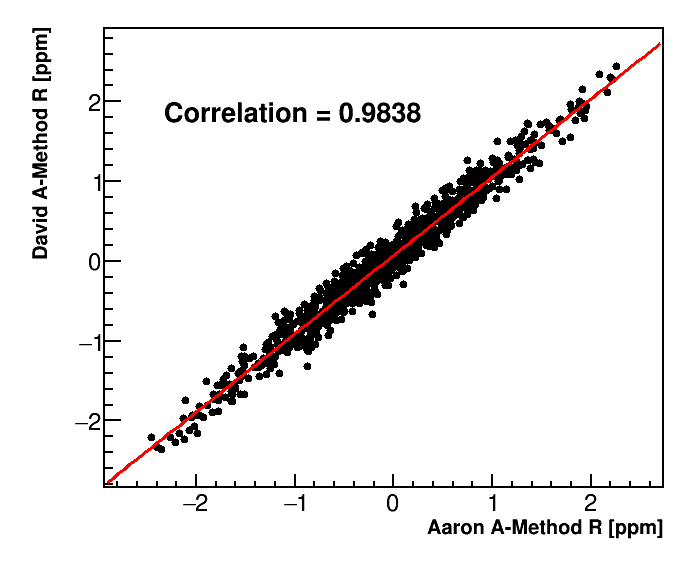
\includegraphics[width=0.6\textwidth]{ScatterPlot}
\caption{Scatter plot between \R values for two different analyses, from jobs submitted for the 9d dataset East-To-West variant. The correlation coefficient between these two analyses is determined from this scatter plot, and the red line simply guides the eye.}
\label{fig:scatterPlot}
\end{figure}


\begin{figure}[]
\centering
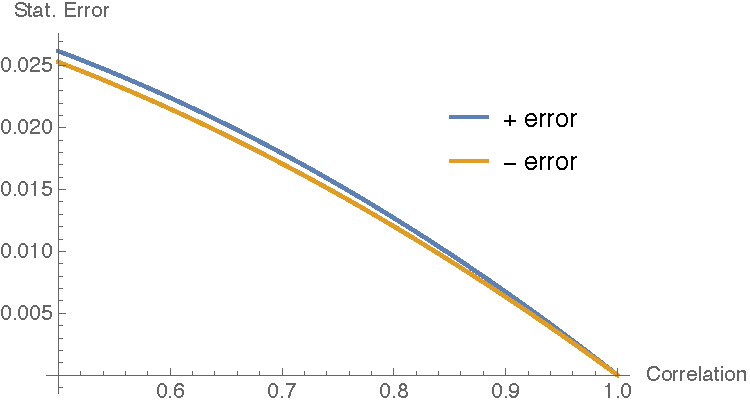
\includegraphics[width=0.6\textwidth]{StatisticalError}
\caption{Statistical error on the correlation coefficient as a function of the correlation, for 851 samples.}
\label{fig:statError}
\end{figure}



The final correlation coefficients are calculated as the average of the correlation coefficients produced with the East-To-West and West-To-East variants. The statistical errors on the correlation coefficients are the averages of the respective statistical errors calculated as described previously. The systematic errors are determined as the difference between the average correlation coefficients and either of the two variants. This systematic error will include it's own statistical error since the two variants come from different job submissions, however the extra error is conservatively simply included in the systematic number. The total error is then the quadrature sum of the statistical and systematic errors as usual. (The errors on the correlation coefficients tend to get smaller as the correlations go up, including the systematic error.)


The correlation matrix between different analyzers for the EG dataset is shown in \figref{fig:corrMatAnalyzer}. Tables for the correlation coefficients and their errors for all four datasets are given in Tables~\ref{tab:Corrs_60h_analyzer} through \ref{tab:Corrs_EG_analyzer}. In general the correlations when compared across datasets are very similar, barring some slight differences in different table entries. In general the differences between datasets don't appear particularly signed one way or another. The correlations between the T and A-Methods are typically around 90\%, between T and Q-Methods is around 50\%, between A and Q-Methods is around 57-60\%, and between T and R-Methods is around 99.6\%. For comparisons between \RE and \RW see \secref{sub:reconcorrelations}.


-summarize some main facets about the correlations and errors



\begin{figure}[]
\centering
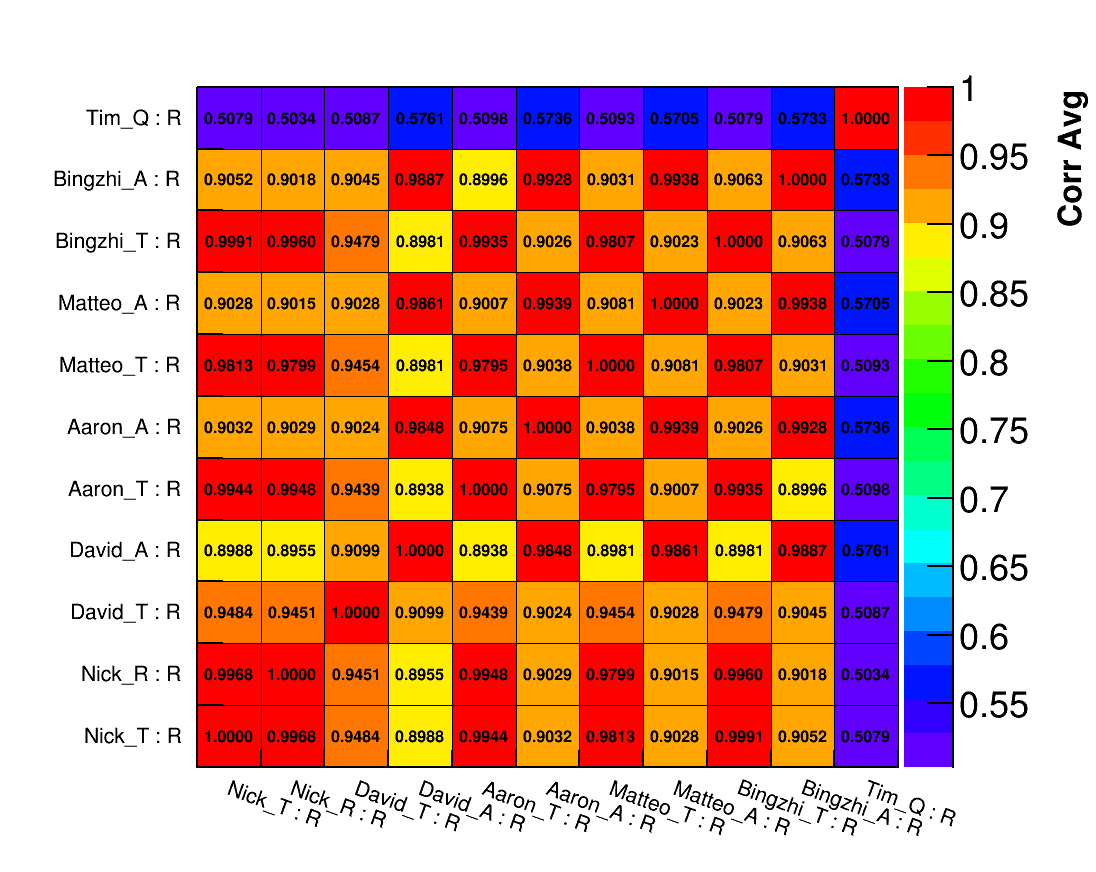
\includegraphics[width=\textwidth]{Avg_CorrelationMatrix_R_R}
\caption{Correlation matrix between different analyzers and methods for the EG dataset. The correlations depicted here are those averaged from the East-To-West and West-To-East variants.}
\label{fig:corrMatAnalyzer}
\end{figure}


% 60h

\begin{landscape}
\begin{table}
\small
\centering
\renewcommand{\arraystretch}{1.5}
\begin{tabularx}{1\linewidth}{@{\extracolsep{\fill}}lXXXXXXXXXXX}
  \toprule
  	\multicolumn{12}{c}{{\normalsize 60h Correlation Coefficients -- Analyzer Level}} \\
  \midrule
  	       & BU T & BU R & CU T & CU A & UW T & UW A & EU T & EU A & SJTU T & SJTU A & UK Q \\
  \midrule
	BU T   & 1.0000 0.0000 & 0.9964 0.0001 & 0.9445 0.0015 & 0.8992 0.0016 & 0.9935 0.0001 & 0.8977 0.0004 & 0.9783 0.0001 & 0.9014 0.0002 & 0.9992 0.0001 & 0.9050 0.0004 & 0.5279 0.0208  \\
	BU R   & 0.9964 0.0001 & 1.0000 0.0000 & 0.9418 0.0018 & 0.8969 0.0020 & 0.9943 0.0001 & 0.8987 0.0008 & 0.9776 0.0004 & 0.9008 0.0007 & 0.9956 0.0001 & 0.9023 0.0010 & 0.5256 0.0203  \\
	CU T   & 0.9445 0.0015 & 0.9418 0.0018 & 1.0000 0.0000 & 0.9043 0.0010 & 0.9395 0.0013 & 0.8933 0.0024 & 0.9399 0.0019 & 0.8963 0.0021 & 0.9436 0.0015 & 0.8992 0.0021 & 0.5248 0.0176  \\
	CU A   & 0.8992 0.0016 & 0.8969 0.0020 & 0.9043 0.0010 & 1.0000 0.0000 & 0.8972 0.0003 & 0.9840 0.0001 & 0.8999 0.0021 & 0.9855 0.0003 & 0.8985 0.0022 & 0.9892 0.0004 & 0.5926 0.0227  \\
	UW T   & 0.9935 0.0001 & 0.9943 0.0001 & 0.9395 0.0013 & 0.8972 0.0003 & 1.0000 0.0000 & 0.9065 0.0010 & 0.9771 0.0001 & 0.9025 0.0012 & 0.9928 0.0001 & 0.9022 0.0010 & 0.5324 0.0229  \\
	UW A   & 0.8977 0.0004 & 0.8987 0.0008 & 0.8933 0.0024 & 0.9840 0.0001 & 0.9065 0.0010 & 1.0000 0.0000 & 0.9016 0.0005 & 0.9933 0.0002 & 0.8971 0.0006 & 0.9916 0.0002 & 0.5927 0.0300  \\
	EU T   & 0.9783 0.0001 & 0.9776 0.0004 & 0.9399 0.0019 & 0.8999 0.0021 & 0.9771 0.0001 & 0.9016 0.0005 & 1.0000 0.0000 & 0.9091 0.0003 & 0.9775 0.0001 & 0.9041 0.0004 & 0.5406 0.0262  \\
	EU A   & 0.9014 0.0002 & 0.9008 0.0007 & 0.8963 0.0021 & 0.9855 0.0003 & 0.9025 0.0012 & 0.9933 0.0002 & 0.9091 0.0003 & 1.0000 0.0000 & 0.9006 0.0004 & 0.9934 0.0001 & 0.5928 0.0306  \\
	SJTU T & 0.9992 0.0001 & 0.9956 0.0001 & 0.9436 0.0015 & 0.8985 0.0022 & 0.9928 0.0001 & 0.8971 0.0006 & 0.9775 0.0001 & 0.9006 0.0004 & 1.0000 0.0000 & 0.9058 0.0007 & 0.5271 0.0202  \\
	SJTU A & 0.9050 0.0004 & 0.9023 0.0010 & 0.8992 0.0021 & 0.9892 0.0004 & 0.9022 0.0010 & 0.9916 0.0002 & 0.9041 0.0004 & 0.9934 0.0001 & 0.9058 0.0007 & 1.0000 0.0000 & 0.5893 0.0274  \\
	UK Q   & 0.5279 0.0208 & 0.5256 0.0203 & 0.5248 0.0176 & 0.5926 0.0227 & 0.5324 0.0229 & 0.5927 0.0300 & 0.5406 0.0262 & 0.5928 0.0306 & 0.5271 0.0202 & 0.5893 0.0274 & 1.0000 0.0000  \\
  \bottomrule
\end{tabularx}
\caption[]{Correlation coefficients between \R values for the 60h dataset, at the analyzer level. In each table cell, the top number is the correlation coefficient and the bottom number is the error on the coefficient.}
\label{tab:Corrs_60h_analyzer}
\end{table}
\end{landscape}

% HK

\begin{landscape}
\begin{table}
\small
\centering
\renewcommand{\arraystretch}{1.5}
\begin{tabularx}{1\linewidth}{@{\extracolsep{\fill}}lXXXXXXXXXXX}
  \toprule
  	\multicolumn{12}{c}{{\normalsize HK Correlation Coefficients -- Analyzer Level}} \\
  \midrule
  	       & BU T & BU R & CU T & CU A & UW T & UW A & EU T & EU A & SJTU T & SJTU A & UK Q \\
  \midrule
	BU T   & 1.0000 0.0000 & 0.9967 0.0001 & 0.9469 0.0023 & 0.8924 0.0042 & 0.9939 0.0003 & 0.8938 0.0015 & 0.9799 0.0011 & 0.8946 0.0031 & 0.9992 0.0001 & 0.8978 0.0033 & 0.4982 0.0057  \\
	BU R   & 0.9967 0.0001 & 1.0000 0.0000 & 0.9439 0.0024 & 0.8907 0.0047 & 0.9943 0.0003 & 0.8955 0.0018 & 0.9785 0.0010 & 0.8948 0.0035 & 0.9958 0.0001 & 0.8959 0.0036 & 0.4959 0.0070  \\
	CU T   & 0.9469 0.0023 & 0.9439 0.0024 & 1.0000 0.0000 & 0.8968 0.0027 & 0.9408 0.0028 & 0.8858 0.0002 & 0.9409 0.0012 & 0.8865 0.0010 & 0.9458 0.0025 & 0.8900 0.0015 & 0.4913 0.0114  \\
	CU A   & 0.8924 0.0042 & 0.8907 0.0047 & 0.8968 0.0027 & 1.0000 0.0000 & 0.8872 0.0058 & 0.9839 0.0010 & 0.8900 0.0026 & 0.9846 0.0004 & 0.8913 0.0045 & 0.9892 0.0003 & 0.5635 0.0137  \\
	UW T   & 0.9939 0.0003 & 0.9943 0.0003 & 0.9408 0.0028 & 0.8872 0.0058 & 1.0000 0.0000 & 0.8993 0.0019 & 0.9776 0.0020 & 0.8928 0.0042 & 0.9930 0.0002 & 0.8920 0.0046 & 0.5015 0.0021  \\
	UW A   & 0.8938 0.0015 & 0.8955 0.0018 & 0.8858 0.0002 & 0.9839 0.0010 & 0.8993 0.0019 & 1.0000 0.0000 & 0.8943 0.0008 & 0.9935 0.0005 & 0.8928 0.0018 & 0.9918 0.0005 & 0.5642 0.0115  \\
	EU T   & 0.9799 0.0011 & 0.9785 0.0010 & 0.9409 0.0012 & 0.8900 0.0026 & 0.9776 0.0020 & 0.8943 0.0008 & 1.0000 0.0000 & 0.8998 0.0014 & 0.9791 0.0012 & 0.8949 0.0018 & 0.5066 0.0020  \\
	EU A   & 0.8946 0.0031 & 0.8948 0.0035 & 0.8865 0.0010 & 0.9846 0.0004 & 0.8928 0.0042 & 0.9935 0.0005 & 0.8998 0.0014 & 1.0000 0.0000 & 0.8936 0.0035 & 0.9935 0.0001 & 0.5637 0.0121  \\
	SJTU T & 0.9992 0.0001 & 0.9958 0.0001 & 0.9458 0.0025 & 0.8913 0.0045 & 0.9930 0.0002 & 0.8928 0.0018 & 0.9791 0.0012 & 0.8936 0.0035 & 1.0000 0.0000 & 0.8984 0.0037 & 0.4987 0.0059  \\
	SJTU A & 0.8978 0.0033 & 0.8959 0.0036 & 0.8900 0.0015 & 0.9892 0.0003 & 0.8920 0.0046 & 0.9918 0.0005 & 0.8949 0.0018 & 0.9935 0.0001 & 0.8984 0.0037 & 1.0000 0.0000 & 0.5612 0.0141  \\
	UK Q   & 0.4982 0.0057 & 0.4959 0.0070 & 0.4913 0.0114 & 0.5635 0.0137 & 0.5015 0.0021 & 0.5642 0.0115 & 0.5066 0.0020 & 0.5637 0.0121 & 0.4987 0.0059 & 0.5612 0.0141 & 1.0000 0.0000  \\
  \bottomrule
\end{tabularx}
\caption[]{Correlation coefficients between \R values for the HK dataset, at the analyzer level. In each table cell, the top number is the correlation coefficient and the bottom number is the error on the coefficient.}
\label{tab:Corrs_HK_analyzer}
\end{table}
\end{landscape}

% 9d

\begin{landscape}
\begin{table}
\small
\centering
\renewcommand{\arraystretch}{1.5}
\begin{tabularx}{1\linewidth}{@{\extracolsep{\fill}}lXXXXXXXXXXX}
  \toprule
  	\multicolumn{12}{c}{{\normalsize 9d Correlation Coefficients -- Analyzer Level}} \\
  \midrule
  	       & BU T & BU R & CU T & CU A & UW T & UW A & EU T & EU A & SJTU T & SJTU A & UK Q \\
  \midrule
	BU T   & 1.0000 0.0000 & 0.9965 0.0003 & 0.9445 0.0015 & 0.8912 0.0087 & 0.9939 0.0005 & 0.8935 0.0058 & 0.9787 0.0018 & 0.8952 0.0082 & 0.9993 0.0001 & 0.8983 0.0071 & 0.4936 0.0105  \\
	BU R   & 0.9965 0.0003 & 1.0000 0.0000 & 0.9414 0.0018 & 0.8885 0.0097 & 0.9944 0.0004 & 0.8944 0.0061 & 0.9782 0.0011 & 0.8945 0.0084 & 0.9958 0.0003 & 0.8957 0.0077 & 0.4888 0.0109  \\
	CU T   & 0.9445 0.0015 & 0.9414 0.0018 & 1.0000 0.0000 & 0.9002 0.0022 & 0.9392 0.0025 & 0.8905 0.0007 & 0.9419 0.0011 & 0.8906 0.0018 & 0.9438 0.0019 & 0.8944 0.0017 & 0.5000 0.0071  \\
	CU A   & 0.8912 0.0087 & 0.8885 0.0097 & 0.9002 0.0022 & 1.0000 0.0000 & 0.8861 0.0102 & 0.9833 0.0005 & 0.8904 0.0059 & 0.9840 0.0005 & 0.8903 0.0090 & 0.9886 0.0006 & 0.5710 0.0007  \\
	UW T   & 0.9939 0.0005 & 0.9944 0.0004 & 0.9392 0.0025 & 0.8861 0.0102 & 1.0000 0.0000 & 0.8990 0.0068 & 0.9770 0.0011 & 0.8931 0.0098 & 0.9931 0.0005 & 0.8929 0.0089 & 0.4999 0.0128  \\
	UW A   & 0.8935 0.0058 & 0.8944 0.0061 & 0.8905 0.0007 & 0.9833 0.0005 & 0.8990 0.0068 & 1.0000 0.0000 & 0.8966 0.0032 & 0.9932 0.0002 & 0.8926 0.0060 & 0.9923 0.0002 & 0.5750 0.0031  \\
	EU T   & 0.9787 0.0018 & 0.9782 0.0011 & 0.9419 0.0011 & 0.8904 0.0059 & 0.9770 0.0011 & 0.8966 0.0032 & 1.0000 0.0000 & 0.9021 0.0056 & 0.9778 0.0019 & 0.8974 0.0053 & 0.4992 0.0042  \\
	EU A   & 0.8952 0.0082 & 0.8945 0.0084 & 0.8906 0.0018 & 0.9840 0.0005 & 0.8931 0.0098 & 0.9932 0.0002 & 0.9021 0.0056 & 1.0000 0.0000 & 0.8944 0.0083 & 0.9940 0.0002 & 0.5698 0.0015  \\
	SJTU T & 0.9993 0.0001 & 0.9958 0.0003 & 0.9438 0.0019 & 0.8903 0.0090 & 0.9931 0.0005 & 0.8926 0.0060 & 0.9778 0.0019 & 0.8944 0.0083 & 1.0000 0.0000 & 0.8988 0.0074 & 0.4913 0.0108  \\
	SJTU A & 0.8983 0.0071 & 0.8957 0.0077 & 0.8944 0.0017 & 0.9886 0.0006 & 0.8929 0.0089 & 0.9923 0.0002 & 0.8974 0.0053 & 0.9940 0.0002 & 0.8988 0.0074 & 1.0000 0.0000 & 0.5651 0.0011  \\
	UK Q   & 0.4936 0.0105 & 0.4888 0.0109 & 0.5000 0.0071 & 0.5710 0.0007 & 0.4999 0.0128 & 0.5750 0.0031 & 0.4992 0.0042 & 0.5698 0.0015 & 0.4913 0.0108 & 0.5651 0.0011 & 1.0000 0.0000  \\
  \bottomrule
\end{tabularx}
\caption[]{Correlation coefficients between \R values for the 9d dataset, at the analyzer level. In each table cell, the top number is the correlation coefficient and the bottom number is the error on the coefficient.}
\label{tab:Corrs_9d_analyzer}
\end{table}
\end{landscape}

% EG

\begin{landscape}
\begin{table}
\small
\centering
\renewcommand{\arraystretch}{1.5}
\begin{tabularx}{1\linewidth}{@{\extracolsep{\fill}}lXXXXXXXXXXX}
  \toprule
  	\multicolumn{12}{c}{{\normalsize EG Correlation Coefficients -- Analyzer Level}} \\
  \midrule
  	       & BU T & BU R & CU T & CU A & UW T & UW A & EU T & EU A & SJTU T & SJTU A & UK Q \\
  \midrule
	BU T   & 1.0000 0.0000 & 0.9968 0.0001 & 0.9484 0.0020 & 0.8988 0.0091 & 0.9944 0.0004 & 0.9032 0.0073 & 0.9813 0.0004 & 0.9028 0.0086 & 0.9991 0.0001 & 0.9052 0.0088 & 0.5079 0.0104  \\
	BU R   & 0.9968 0.0001 & 1.0000 0.0000 & 0.9451 0.0025 & 0.8955 0.0102 & 0.9948 0.0006 & 0.9029 0.0087 & 0.9799 0.0007 & 0.9015 0.0096 & 0.9960 0.0001 & 0.9018 0.0099 & 0.5034 0.0099  \\
	CU T   & 0.9484 0.0020 & 0.9451 0.0025 & 1.0000 0.0000 & 0.9099 0.0025 & 0.9439 0.0019 & 0.9024 0.0008 & 0.9454 0.0032 & 0.9028 0.0010 & 0.9479 0.0016 & 0.9045 0.0005 & 0.5087 0.0090  \\
	CU A   & 0.8988 0.0091 & 0.8955 0.0102 & 0.9099 0.0025 & 1.0000 0.0000 & 0.8938 0.0099 & 0.9848 0.0005 & 0.8981 0.0105 & 0.9861 0.0002 & 0.8981 0.0092 & 0.9887 0.0006 & 0.5761 0.0012  \\
	UW T   & 0.9944 0.0004 & 0.9948 0.0006 & 0.9439 0.0019 & 0.8938 0.0099 & 1.0000 0.0000 & 0.9075 0.0079 & 0.9795 0.0010 & 0.9007 0.0095 & 0.9935 0.0005 & 0.8996 0.0100 & 0.5098 0.0102  \\
	UW A   & 0.9032 0.0073 & 0.9029 0.0087 & 0.9024 0.0008 & 0.9848 0.0005 & 0.9075 0.0079 & 1.0000 0.0000 & 0.9038 0.0088 & 0.9939 0.0004 & 0.9026 0.0072 & 0.9928 0.0004 & 0.5736 0.0038  \\
	EU T   & 0.9813 0.0004 & 0.9799 0.0007 & 0.9454 0.0032 & 0.8981 0.0105 & 0.9795 0.0010 & 0.9038 0.0088 & 1.0000 0.0000 & 0.9081 0.0096 & 0.9807 0.0004 & 0.9031 0.0096 & 0.5093 0.0083  \\
	EU A   & 0.9028 0.0086 & 0.9015 0.0096 & 0.9028 0.0010 & 0.9861 0.0002 & 0.9007 0.0095 & 0.9939 0.0004 & 0.9081 0.0096 & 1.0000 0.0000 & 0.9023 0.0086 & 0.9938 0.0002 & 0.5705 0.0034  \\
	SJTU T & 0.9991 0.0001 & 0.9960 0.0001 & 0.9479 0.0016 & 0.8981 0.0092 & 0.9935 0.0005 & 0.9026 0.0072 & 0.9807 0.0004 & 0.9023 0.0086 & 1.0000 0.0000 & 0.9063 0.0086 & 0.5079 0.0110  \\
	SJTU A & 0.9052 0.0088 & 0.9018 0.0099 & 0.9045 0.0005 & 0.9887 0.0006 & 0.8996 0.0100 & 0.9928 0.0004 & 0.9031 0.0096 & 0.9938 0.0002 & 0.9063 0.0086 & 1.0000 0.0000 & 0.5733 0.0013  \\
	UK Q   & 0.5079 0.0104 & 0.5034 0.0099 & 0.5087 0.0090 & 0.5761 0.0012 & 0.5098 0.0102 & 0.5736 0.0038 & 0.5093 0.0083 & 0.5705 0.0034 & 0.5079 0.0110 & 0.5733 0.0013 & 1.0000 0.0000  \\
  \bottomrule
\end{tabularx}
\caption[]{Correlation coefficients between \R values for the EG dataset, at the analyzer level. In each table cell, the top number is the correlation coefficient and the bottom number is the error on the coefficient.}
\label{tab:Corrs_EG_analyzer}
\end{table}
\end{landscape}



\subsection{Sigma Differences}

% -maybe use the word pull instead of sigma here somehow?


Once the correlations between the different analyses and methods have been determined, the significance of the differences in results between those analyses can be determined. \tabref{tab:analysisRValues} gives the commonly blinded fitted \R values for the different datasets and different analyses along with their errors. The $1\sigma$ allowed deviation between two analysis results is given by
\begin{align}
	\sigma_{\text{allowed}} = \sqrt{\sigma^{2}_{i} + \sigma^{2}_{j} - 2r_{ij}\sigma_{i}\sigma_{j}}
\end{align}
where $\sigma_{i}$ and $\sigma_{j}$ are the errors of the two analyses, and $r_{ij}$ is the correlation coefficient between the two analyses. Using this equation and the provided correlation coefficients, the allowed differences between all of the analyses for the four datasets are determined. Tables~\ref{tab:60h_diff} through \ref{tab:EG_diff} display the allowed differences in ppb between the different analyses, as well as the number of $\sigma$s difference or `pull' after calculating the $\Delta R$s from \tabref{tab:analysisRValues}.  In general the deviations between the different analyses are spread around 0 with deviations rising into the two sigma range. Some specifics to note are that the Q-Method fits in the HK and 9d datasets are something like $1.35\sigma$ or so above the rest depending on the exact correlation, and the R-Method values are consistently below low the rest barring a few entries, up to around $2\sigma$ or so in some cases. In order to get a sense of the spread of pulls, all entries from the top-side of the diagonal were taken for each of the datasets and put into a histogram, as shown in \figref{fig:AllSigmas}. The resulting distribution while not perfect shows a nice symmetry around 0, with few entries close to $2\sigma$ or higher. This histogram provides some confidence that the differences are natural and to be expected.


% -make sure I use the same notation for the correlation coefficients everywhere, r probably


\begin{table}
\small
\centering
\renewcommand{\arraystretch}{1.2}
\begin{tabularx}{1\linewidth}{@{\extracolsep{\fill}}lcccccccc}
  \toprule
  	\multicolumn{9}{c}{{\normalsize \Rone Commonly Blinded Results }} \\
  \midrule
  	\multirow{2}{*}{Analysis} & \multicolumn{2}{c}{60h} & \multicolumn{2}{c}{HK} & \multicolumn{2}{c}{9d} & \multicolumn{2}{c}{EG} \\ \cmidrule{2-3} \cmidrule{4-5} \cmidrule{6-7} \cmidrule{8-9}
  			 & \R & $\sigma_{R}$ & \R & $\sigma_{R}$ & \R & $\sigma_{R}$ & \R & $\sigma_{R}$ \\
  \midrule
	BU T   & $-28.8023$ & 1.3582 & $-27.0442$ & 1.1561 & $-27.9171$ & 0.9301 & $-27.7020$ & 0.7584 \\
	BU R   & $-28.9668$ & 1.3598 & $-27.2093$ & 1.1574 & $-27.9218$ & 0.9327 & $-27.7654$ & 0.7576 \\
	CU T   & $-28.2111$ & 1.3377 & $-27.2093$ & 1.1336 & $-28.0202$ & 0.9126 & $-27.7152$ & 0.7474 \\
	CU A   & $-28.2288$ & 1.2079 & $-26.9466$ & 1.0234 & $-27.5532$ & 0.8240 & $-27.5902$ & 0.6758 \\
	UW T   & $-28.6199$ & 1.3308 & $-27.0049$ & 1.1277 & $-27.8989$ & 0.9079 & $-27.7144$ & 0.7437 \\
	UW A   & $-28.6373$ & 1.2184 & $-26.9657$ & 1.0302 & $-27.5723$ & 0.8305 & $-27.6694$ & 0.6799 \\
	EU T   & $-28.8848$ & 1.3327 & $-27.0806$ & 1.1203 & $-27.8890$ & 0.9067 & $-27.8772$ & 0.7435 \\
	EU A   & $-28.4813$ & 1.1938 & $-27.0213$ & 1.0120 & $-27.5998$ & 0.8146 & $-27.7276$ & 0.6679 \\
	SJTU T & $-28.7398$ & 1.3314 & $-27.0019$ & 1.1281 & $-27.8935$ & 0.9084 & $-27.6658$ & 0.7441 \\
	SJTU A & $-28.4228$ & 1.2061 & $-27.0910$ & 1.0223 & $-27.7440$ & 0.8224 & $-27.6945$ & 0.6729 \\
	UK Q   & $-29.2062$ & 2.0585 & $-24.9464$ & 1.7478 & $-26.2794$ & 1.4032 & $-27.9905$ & 1.2690 \\
  \bottomrule
\end{tabularx}
\caption[]{Fit results for \R and it's error for the different \Rone datasets and analyses. \R here is commonly blinded, and still contains both a software and hardware blinding.}
\label{tab:analysisRValues}
\end{table}





\begin{landscape}
\begin{table}
\small
\centering
\renewcommand{\arraystretch}{1.5}
\begin{tabularx}{1\linewidth}{@{\extracolsep{\fill}}lXXXXXXXXXXX}
  \toprule
  	\multicolumn{12}{c}{{\normalsize 60h Analysis Differences}} \\
  \midrule
  	       & BU T & BU R & CU T & CU A & UW T & UW A & EU T & EU A & SJTU T & SJTU A & UK Q \\
  \midrule
	BU T   & 0.0000 $+0.00$ & 0.1154 $-1.42$ & 0.4495 $+1.32$ & 0.5943 $+0.96$ & 0.1555 $+1.17$ & 0.5983 $+0.28$ & 0.2817 $-0.29$ & 0.5890 $+0.55$ & 0.0609 $+1.03$ & 0.5781 $+0.66$ & 1.7692 $-0.23$  \\
	BU R   & 0.1154 $+1.42$ & 0.0000 $+0.00$ & 0.4609 $+1.64$ & 0.6015 $+1.23$ & 0.1464 $+2.37$ & 0.5963 $+0.55$ & 0.2862 $+0.29$ & 0.5912 $+0.82$ & 0.1288 $+1.76$ & 0.5867 $+0.93$ & 1.7731 $-0.14$  \\
	CU T   & 0.4495 $-1.32$ & 0.4609 $-1.64$ & 0.0000 $+0.00$ & 0.5710 $-0.03$ & 0.4642 $-0.88$ & 0.6017 $-0.71$ & 0.4628 $-1.46$ & 0.5933 $-0.46$ & 0.4484 $-1.18$ & 0.5854 $-0.36$ & 1.7710 $-0.56$  \\
	CU A   & 0.5943 $-0.96$ & 0.6015 $-1.23$ & 0.5710 $+0.03$ & 0.0000 $+0.00$ & 0.5879 $-0.67$ & 0.2172 $-1.88$ & 0.5813 $-1.13$ & 0.2050 $-1.23$ & 0.5846 $-0.87$ & 0.1774 $-1.09$ & 1.6581 $-0.59$  \\
	UW T   & 0.1555 $-1.17$ & 0.1464 $-2.37$ & 0.4642 $+0.88$ & 0.5879 $+0.67$ & 0.0000 $+0.00$ & 0.5619 $-0.03$ & 0.2851 $-0.93$ & 0.5731 $+0.24$ & 0.1600 $-0.75$ & 0.5741 $+0.34$ & 1.7583 $-0.33$  \\
	UW A   & 0.5983 $-0.28$ & 0.5963 $-0.55$ & 0.6017 $+0.71$ & 0.2172 $+1.88$ & 0.5619 $+0.03$ & 0.0000 $+0.00$ & 0.5767 $-0.43$ & 0.1419 $+1.10$ & 0.5888 $-0.17$ & 0.1572 $+1.36$ & 1.6580 $-0.34$  \\
	EU T   & 0.2817 $+0.29$ & 0.2862 $-0.29$ & 0.4628 $+1.46$ & 0.5813 $+1.13$ & 0.2851 $+0.93$ & 0.5767 $+0.43$ & 0.0000 $+0.00$ & 0.5553 $+0.73$ & 0.2827 $+0.51$ & 0.5696 $+0.81$ & 1.7456 $-0.18$  \\
	EU A   & 0.5890 $-0.55$ & 0.5912 $-0.82$ & 0.5933 $+0.46$ & 0.2050 $+1.23$ & 0.5731 $-0.24$ & 0.1419 $-1.10$ & 0.5553 $-0.73$ & 0.0000 $+0.00$ & 0.5786 $-0.45$ & 0.1389 $+0.42$ & 1.6580 $-0.44$  \\
	SJTU T & 0.0609 $-1.03$ & 0.1288 $-1.76$ & 0.4484 $+1.18$ & 0.5846 $+0.87$ & 0.1600 $+0.75$ & 0.5888 $+0.17$ & 0.2827 $-0.51$ & 0.5786 $+0.45$ & 0.0000 $+0.00$ & 0.5641 $+0.56$ & 1.7665 $-0.26$  \\
	SJTU A & 0.5781 $-0.66$ & 0.5867 $-0.93$ & 0.5854 $+0.36$ & 0.1774 $+1.09$ & 0.5741 $-0.34$ & 0.1572 $-1.36$ & 0.5696 $-0.81$ & 0.1389 $-0.42$ & 0.5641 $-0.56$ & 0.0000 $+0.00$ & 1.6632 $-0.47$  \\
	UK Q   & 1.7692 $+0.23$ & 1.7731 $+0.14$ & 1.7710 $+0.56$ & 1.6581 $+0.59$ & 1.7583 $+0.33$ & 1.6580 $+0.34$ & 1.7456 $+0.18$ & 1.6580 $+0.44$ & 1.7665 $+0.26$ & 1.6632 $+0.47$ & 0.0000 $+0.00$  \\
  \bottomrule
\end{tabularx}
\caption[]{Differences in \R values for the 60h dataset between the different analyses. The top number is the allowed ppb difference in \R, $\sigma_{\text{allowed}}$, as calculated from the correlation coefficients and analysis errors. The bottom number is the number of sigmas difference, calculated as $\sigma_{\text{diff}} = (R_{\text{column}}-R_{\text{row}})/\sigma_{\text{allowed}}$.}
\label{tab:60h_diff}
\end{table}
\end{landscape}




\begin{landscape}
\begin{table}
\small
\centering
\renewcommand{\arraystretch}{1.5}
\begin{tabularx}{1\linewidth}{@{\extracolsep{\fill}}lXXXXXXXXXXX}
  \toprule
  	\multicolumn{12}{c}{{\normalsize HK Analysis Differences}} \\
  \midrule
  	       & BU T & BU R & CU T & CU A & UW T & UW A & EU T & EU A & SJTU T & SJTU A & UK Q \\
  \midrule
	BU T   & 0.0000 $+0.00$ & 0.0943 $-1.75$ & 0.3736 $-0.44$ & 0.5218 $+0.19$ & 0.1293 $+0.30$ & 0.5184 $+0.15$ & 0.2310 $-0.16$ & 0.5172 $+0.04$ & 0.0544 $+0.78$ & 0.5094 $-0.09$ & 1.5421 $+1.36$  \\
	BU R   & 0.0943 $+1.75$ & 0.0000 $+0.00$ & 0.3846 $-0.00$ & 0.5262 $+0.50$ & 0.1256 $+1.63$ & 0.5153 $+0.47$ & 0.2389 $+0.54$ & 0.5172 $+0.36$ & 0.1087 $+1.91$ & 0.5143 $+0.23$ & 1.5454 $+1.46$  \\
	CU T   & 0.3736 $+0.44$ & 0.3846 $+0.00$ & 0.0000 $+0.00$ & 0.5015 $+0.52$ & 0.3891 $+0.53$ & 0.5267 $+0.46$ & 0.3878 $+0.33$ & 0.5246 $+0.36$ & 0.3724 $+0.56$ & 0.5169 $+0.23$ & 1.5470 $+1.46$  \\
	CU A   & 0.5218 $-0.19$ & 0.5262 $-0.50$ & 0.5015 $-0.52$ & 0.0000 $+0.00$ & 0.5208 $-0.11$ & 0.1842 $-0.10$ & 0.5114 $-0.26$ & 0.1788 $-0.42$ & 0.5119 $-0.11$ & 0.1502 $-0.96$ & 1.4443 $+1.38$  \\
	UW T   & 0.1293 $-0.30$ & 0.1256 $-1.63$ & 0.3891 $-0.53$ & 0.5208 $+0.11$ & 0.0000 $+0.00$ & 0.4934 $+0.08$ & 0.2380 $-0.32$ & 0.5080 $-0.03$ & 0.1338 $+0.02$ & 0.5101 $-0.17$ & 1.5328 $+1.34$  \\
	UW A   & 0.5184 $-0.15$ & 0.5153 $-0.47$ & 0.5267 $-0.46$ & 0.1842 $+0.10$ & 0.4934 $-0.08$ & 0.0000 $+0.00$ & 0.5022 $-0.23$ & 0.1181 $-0.47$ & 0.5086 $-0.07$ & 0.1314 $-0.95$ & 1.4438 $+1.40$  \\
	EU T   & 0.2310 $+0.16$ & 0.2389 $-0.54$ & 0.3878 $-0.33$ & 0.5114 $+0.26$ & 0.2380 $+0.32$ & 0.5022 $+0.23$ & 0.0000 $+0.00$ & 0.4888 $+0.12$ & 0.2301 $+0.34$ & 0.5004 $-0.02$ & 1.5251 $+1.40$  \\
	EU A   & 0.5172 $-0.04$ & 0.5172 $-0.36$ & 0.5246 $-0.36$ & 0.1788 $+0.42$ & 0.5080 $+0.03$ & 0.1181 $+0.47$ & 0.4888 $-0.12$ & 0.0000 $+0.00$ & 0.5064 $+0.04$ & 0.1163 $-0.60$ & 1.4439 $+1.44$  \\
	SJTU T & 0.0544 $-0.78$ & 0.1087 $-1.91$ & 0.3724 $-0.56$ & 0.5119 $+0.11$ & 0.1338 $-0.02$ & 0.5086 $+0.07$ & 0.2301 $-0.34$ & 0.5064 $-0.04$ & 0.0000 $+0.00$ & 0.4956 $-0.18$ & 1.5365 $+1.34$  \\
	SJTU A & 0.5094 $+0.09$ & 0.5143 $-0.23$ & 0.5169 $-0.23$ & 0.1502 $+0.96$ & 0.5101 $+0.17$ & 0.1314 $+0.95$ & 0.5004 $+0.02$ & 0.1163 $+0.60$ & 0.4956 $+0.18$ & 0.0000 $+0.00$ & 1.4472 $+1.48$  \\
	UK Q   & 1.5421 $-1.36$ & 1.5454 $-1.46$ & 1.5470 $-1.46$ & 1.4443 $-1.38$ & 1.5328 $-1.34$ & 1.4438 $-1.40$ & 1.5251 $-1.40$ & 1.4439 $-1.44$ & 1.5365 $-1.34$ & 1.4472 $-1.48$ & 0.0000 $+0.00$  \\
  \bottomrule
\end{tabularx}
\caption[]{Differences in \R values for the HK dataset between the different analyses. The top number is the allowed ppb difference in \R, $\sigma_{\text{allowed}}$, as calculated from the correlation coefficients and analysis errors. The bottom number is the number of sigmas difference, calculated as $\sigma_{\text{diff}} = (R_{\text{column}}-R_{\text{row}})/\sigma_{\text{allowed}}$.}
\label{tab:HK_diff}
\end{table}
\end{landscape}



\begin{landscape}
\begin{table}
\small
\centering
\renewcommand{\arraystretch}{1.5}
\begin{tabularx}{1\linewidth}{@{\extracolsep{\fill}}lXXXXXXXXXXX}
  \toprule
  	\multicolumn{12}{c}{{\normalsize 9d Analysis Differences}} \\
  \midrule
  	       & BU T & BU R & CU T & CU A & UW T & UW A & EU T & EU A & SJTU T & SJTU A & UK Q \\
  \midrule
	BU T   & 0.0000 $+0.00$ & 0.0775 $-0.06$ & 0.3076 $-0.34$ & 0.4220 $+0.86$ & 0.1040 $+0.17$ & 0.4177 $+0.83$ & 0.1911 $+0.15$ & 0.4148 $+0.76$ & 0.0415 $+0.57$ & 0.4088 $+0.42$ & 1.2432 $+1.32$  \\
	BU R   & 0.0775 $+0.06$ & 0.0000 $+0.00$ & 0.3164 $-0.31$ & 0.4281 $+0.86$ & 0.1007 $+0.23$ & 0.4171 $+0.84$ & 0.1940 $+0.17$ & 0.4174 $+0.77$ & 0.0874 $+0.32$ & 0.4149 $+0.43$ & 1.2487 $+1.32$  \\
	CU T   & 0.3076 $+0.34$ & 0.3164 $+0.31$ & 0.0000 $+0.00$ & 0.3974 $+1.18$ & 0.3175 $+0.38$ & 0.4156 $+1.08$ & 0.3100 $+0.42$ & 0.4151 $+1.01$ & 0.3052 $+0.42$ & 0.4083 $+0.68$ & 1.2334 $+1.41$  \\
	CU A   & 0.4220 $-0.86$ & 0.4281 $-0.86$ & 0.3974 $-1.18$ & 0.0000 $+0.00$ & 0.4213 $-0.82$ & 0.1513 $-0.13$ & 0.4130 $-0.81$ & 0.1469 $-0.32$ & 0.4139 $-0.82$ & 0.1241 $-1.54$ & 1.1522 $+1.11$  \\
	UW T   & 0.1040 $-0.17$ & 0.1007 $-0.23$ & 0.3175 $-0.38$ & 0.4213 $+0.82$ & 0.0000 $+0.00$ & 0.3978 $+0.82$ & 0.1948 $+0.05$ & 0.4085 $+0.73$ & 0.1067 $+0.05$ & 0.4089 $+0.38$ & 1.2327 $+1.31$  \\
	UW A   & 0.4177 $-0.83$ & 0.4171 $-0.84$ & 0.4156 $-1.08$ & 0.1513 $+0.13$ & 0.3978 $-0.82$ & 0.0000 $+0.00$ & 0.4019 $-0.79$ & 0.0973 $-0.28$ & 0.4100 $-0.78$ & 0.1031 $-1.67$ & 1.1483 $+1.13$  \\
	EU T   & 0.1911 $-0.15$ & 0.1940 $-0.17$ & 0.3100 $-0.42$ & 0.4130 $+0.81$ & 0.1948 $-0.05$ & 0.4019 $+0.79$ & 0.0000 $+0.00$ & 0.3912 $+0.74$ & 0.1911 $-0.02$ & 0.4002 $+0.36$ & 1.2332 $+1.31$  \\
	EU A   & 0.4148 $-0.76$ & 0.4174 $-0.77$ & 0.4151 $-1.01$ & 0.1469 $+0.32$ & 0.4085 $-0.73$ & 0.0973 $+0.28$ & 0.3912 $-0.74$ & 0.0000 $+0.00$ & 0.4062 $-0.72$ & 0.0900 $-1.60$ & 1.1532 $+1.14$  \\
	SJTU T & 0.0415 $-0.57$ & 0.0874 $-0.32$ & 0.3052 $-0.42$ & 0.4139 $+0.82$ & 0.1067 $-0.05$ & 0.4100 $+0.78$ & 0.1911 $+0.02$ & 0.4062 $+0.72$ & 0.0000 $+0.00$ & 0.3982 $+0.38$ & 1.2417 $+1.30$  \\
	SJTU A & 0.4088 $-0.42$ & 0.4149 $-0.43$ & 0.4083 $-0.68$ & 0.1241 $+1.54$ & 0.4089 $-0.38$ & 0.1031 $+1.67$ & 0.4002 $-0.36$ & 0.0900 $+1.60$ & 0.3982 $-0.38$ & 0.0000 $+0.00$ & 1.1581 $+1.26$  \\
	UK Q   & 1.2432 $-1.32$ & 1.2487 $-1.32$ & 1.2334 $-1.41$ & 1.1522 $-1.11$ & 1.2327 $-1.31$ & 1.1483 $-1.13$ & 1.2332 $-1.31$ & 1.1532 $-1.14$ & 1.2417 $-1.30$ & 1.1581 $-1.26$ & 0.0000 $+0.00$  \\
  \bottomrule
\end{tabularx}
\caption[]{Differences in \R values for the 9d dataset between the different analyses. The top number is the allowed ppb difference in \R, $\sigma_{\text{allowed}}$, as calculated from the correlation coefficients and analysis errors. The bottom number is the number of sigmas difference, calculated as $\sigma_{\text{diff}} = (R_{\text{column}}-R_{\text{row}})/\sigma_{\text{allowed}}$.}
\label{tab:9d_diff}
\end{table}
\end{landscape}




\begin{landscape}
\begin{table}
\small
\centering
\renewcommand{\arraystretch}{1.5}
\begin{tabularx}{1\linewidth}{@{\extracolsep{\fill}}lXXXXXXXXXXX}
  \toprule
  	\multicolumn{12}{c}{{\normalsize EG Analysis Differences}} \\
  \midrule
  	       & BU T & BU R & CU T & CU A & UW T & UW A & EU T & EU A & SJTU T & SJTU A & UK Q \\
  \midrule
	BU T   & 0.0000 $+0.00$ & 0.0602 $-1.05$ & 0.2421 $-0.05$ & 0.3325 $+0.34$ & 0.0806 $-0.15$ & 0.3256 $+0.10$ & 0.1461 $-1.20$ & 0.3266 $-0.08$ & 0.0346 $+1.04$ & 0.3226 $+0.02$ & 1.0990 $-0.26$  \\
	BU R   & 0.0602 $+1.05$ & 0.0000 $+0.00$ & 0.2495 $+0.20$ & 0.3372 $+0.52$ & 0.0781 $+0.65$ & 0.3257 $+0.29$ & 0.1513 $-0.74$ & 0.3282 $+0.12$ & 0.0687 $+1.45$ & 0.3276 $+0.22$ & 1.1029 $-0.20$  \\
	CU T   & 0.2421 $+0.05$ & 0.2495 $-0.20$ & 0.0000 $+0.00$ & 0.3100 $+0.40$ & 0.2497 $+0.00$ & 0.3221 $+0.14$ & 0.2464 $-0.66$ & 0.3215 $-0.04$ & 0.2409 $+0.21$ & 0.3188 $+0.07$ & 1.0972 $-0.25$  \\
	CU A   & 0.3325 $-0.34$ & 0.3372 $-0.52$ & 0.3100 $-0.40$ & 0.0000 $+0.00$ & 0.3337 $-0.37$ & 0.1183 $-0.67$ & 0.3270 $-0.88$ & 0.1122 $-1.22$ & 0.3274 $-0.23$ & 0.1012 $-1.03$ & 1.0387 $-0.39$  \\
	UW T   & 0.0806 $+0.15$ & 0.0781 $-0.65$ & 0.2497 $-0.00$ & 0.3337 $+0.37$ & 0.0000 $+0.00$ & 0.3125 $+0.14$ & 0.1505 $-1.08$ & 0.3230 $-0.04$ & 0.0851 $+0.57$ & 0.3249 $+0.06$ & 1.0960 $-0.25$  \\
	UW A   & 0.3256 $-0.10$ & 0.3257 $-0.29$ & 0.3221 $-0.14$ & 0.1183 $+0.67$ & 0.3125 $-0.14$ & 0.0000 $+0.00$ & 0.3182 $-0.65$ & 0.0751 $-0.77$ & 0.3204 $+0.01$ & 0.0816 $-0.31$ & 1.0406 $-0.31$  \\
	EU T   & 0.1461 $+1.20$ & 0.1513 $+0.74$ & 0.2464 $+0.66$ & 0.3270 $+0.88$ & 0.1505 $+1.08$ & 0.3182 $+0.65$ & 0.0000 $+0.00$ & 0.3115 $+0.48$ & 0.1460 $+1.45$ & 0.3193 $+0.57$ & 1.0964 $-0.10$  \\
	EU A   & 0.3266 $+0.08$ & 0.3282 $-0.12$ & 0.3215 $+0.04$ & 0.1122 $+1.22$ & 0.3230 $+0.04$ & 0.0751 $+0.77$ & 0.3115 $-0.48$ & 0.0000 $+0.00$ & 0.3208 $+0.19$ & 0.0746 $+0.44$ & 1.0437 $-0.25$  \\
	SJTU T & 0.0346 $-1.04$ & 0.0687 $-1.45$ & 0.2409 $-0.21$ & 0.3274 $+0.23$ & 0.0851 $-0.57$ & 0.3204 $-0.01$ & 0.1460 $-1.45$ & 0.3208 $-0.19$ & 0.0000 $+0.00$ & 0.3145 $-0.09$ & 1.0977 $-0.30$  \\
	SJTU A & 0.3226 $-0.02$ & 0.3276 $-0.22$ & 0.3188 $-0.07$ & 0.1012 $+1.03$ & 0.3249 $-0.06$ & 0.0816 $+0.31$ & 0.3193 $-0.57$ & 0.0746 $-0.44$ & 0.3145 $+0.09$ & 0.0000 $+0.00$ & 1.0411 $-0.28$  \\
	UK Q   & 1.0990 $+0.26$ & 1.1029 $+0.20$ & 1.0972 $+0.25$ & 1.0387 $+0.39$ & 1.0960 $+0.25$ & 1.0406 $+0.31$ & 1.0964 $+0.10$ & 1.0437 $+0.25$ & 1.0977 $+0.30$ & 1.0411 $+0.28$ & 0.0000 $+0.00$  \\
  \bottomrule
\end{tabularx}
\caption[]{Differences in \R values for the EG dataset between the different analyses. The top number is the allowed ppb difference in \R, $\sigma_{\text{allowed}}$, as calculated from the correlation coefficients and analysis errors. The bottom number is the number of sigmas difference, calculated as $\sigma_{\text{diff}} = (R_{\text{column}}-R_{\text{row}})/\sigma_{\text{allowed}}$.}
\label{tab:EG_diff}
\end{table}
\end{landscape}






\begin{figure}[]
\centering
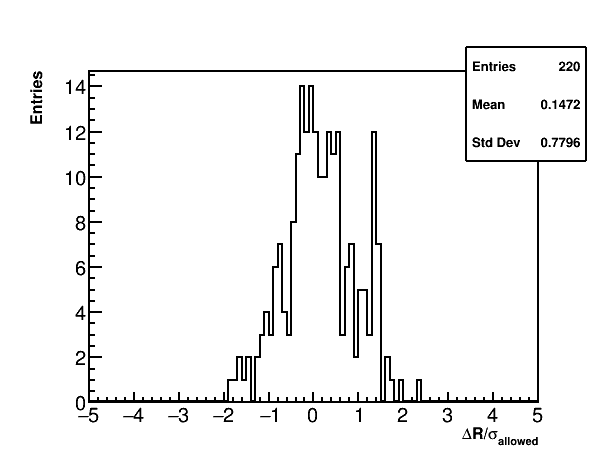
\includegraphics[width=0.65\textwidth]{AllSigmas}
\caption{Sigma diffs from all datasets for the individual analysis comparisons. Identical but oppposite entries from across the main diagonal are not included, as well as the entries for the diagonals themselves. The entries from the top-right of the diagonal are taken and filled into this histogram. In general such a pull distribution should be a unit Gaussian, however entries from the same row or column will be correlated, and are nevertheless included in this plot. This is particularly apparent with the spike around $1.35\sigma$, which comes from some of the Q-Method correlations in the HK and 9d datasets, in both of which the Q-Method fit returned a greater R-value than the rest of the fits. A number of the entries at the high side of the distribution correspond to R-Method fits compared to the rest. These pull the distributions mean to a value greater than 0.}
\label{fig:AllSigmas}
\end{figure}




\clearpage
\subsection{Reconstruction Level Correlations}
\label{sub:reconcorrelations}

In the proposed combination approach (cite David's collaboration talk here or task force discussion?), the correlation coefficients between the different reconstructions are needed. In order to determine these the \R values between the \RW T and A-Methods were averaged among the four and three different analyses respectively, before populating the scatter plots and determining the correlation coefficients\footnote{It should be noted as well that other combinations of different methods, with different averaging on the \R paramaters, were made in order to provide varying correlation coefficients for the combination procedure to give a scale of different numbers for different results.}. The correlation matrix for the EG dataset at the reconstruction level is shown in \figref{fig:corrMatRecon}. Tables~\ref{tab:Corrs_60h_recon} through \ref{tab:Corrs_EG_recon} give the correlations and the errors on the correlations for all four datasets. The correlation between the \RE and \RW T-Methods is around the 95\% level, while that for the A-Methods is around the 98.8\% level. For the A-Method comparison errors, the errors are all less than 0.1\%.



\begin{figure}[]
\centering
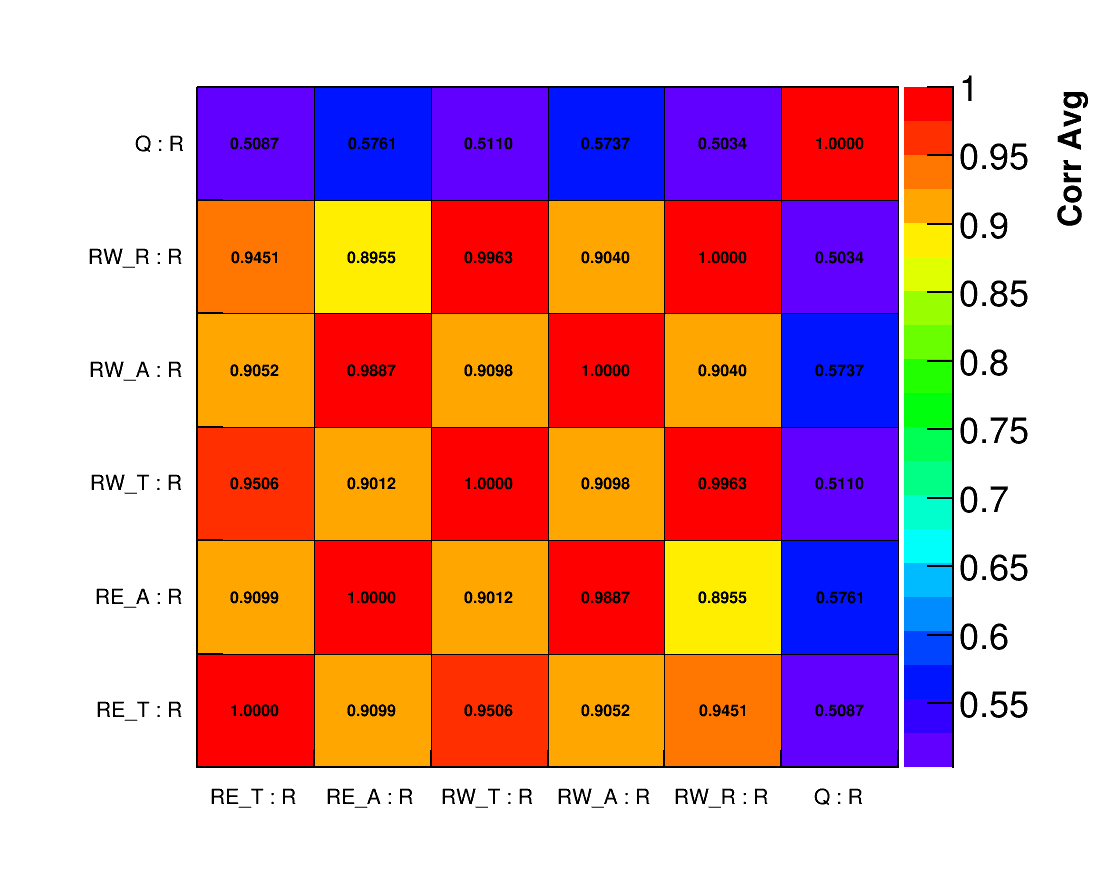
\includegraphics[width=\textwidth]{Avg_Recon_CorrelationMatrix_R_R}
\caption{Correlation matrix between different reconstructions and methods for the EG dataset. The correlations depicted here are those averaged from the East-To-West and West-To-East variants. The \RE, R-Method, and Q-Method analyses are exactly the same as those in the other results tables since there was only one analysis in each of those cases. The \RW T and A-Method results were averaged among the four and three different analyses respectively.}
\label{fig:corrMatRecon}
\end{figure}



\begin{table}
\setlength\tabcolsep{15pt}
\small
\centering
\renewcommand{\arraystretch}{1.4}
\begin{tabularx}{0.8\linewidth}{@{\extracolsep{\fill}}lXXXXXX}
  \toprule
  	\multicolumn{7}{c}{{\normalsize 60h Correlation Coefficients -- Recon. Level}} \\
  \midrule
  	       & RE T & RE A & RW T & RW A & RW R & \quad Q \\
  \midrule
	RE T   & 1.0000 0.0000 & 0.9043 0.0010 & 0.9467 0.0016 & 0.8984 0.0022 & 0.9418 0.0018 & 0.5248 0.0176  \\
	RE A   & 0.9043 0.0010 & 1.0000 0.0000 & 0.9033 0.0015 & 0.9886 0.0002 & 0.8969 0.0020 & 0.5926 0.0227  \\
	RW T   & 0.9467 0.0016 & 0.9033 0.0015 & 1.0000 0.0000 & 0.9097 0.0002 & 0.9961 0.0001 & 0.5348 0.0227  \\
	RW A   & 0.8984 0.0022 & 0.9886 0.0002 & 0.9097 0.0002 & 1.0000 0.0000 & 0.9028 0.0008 & 0.5930 0.0294  \\
	RW R   & 0.9418 0.0018 & 0.8969 0.0020 & 0.9961 0.0001 & 0.9028 0.0008 & 1.0000 0.0000 & 0.5256 0.0203  \\
	Q      & 0.5248 0.0176 & 0.5926 0.0227 & 0.5348 0.0227 & 0.5930 0.0294 & 0.5256 0.0203 & 1.0000 0.0000  \\
  \bottomrule
\end{tabularx}
\caption[]{Correlation coefficients between \R values for the 60h dataset, at the reconstruction level after the \RW T-Method and A-Method \R values were averaged among the different analyzers. In each table cell, the top number is the correlation coefficient and the bottom number is the error on the coefficient.}
\label{tab:Corrs_60h_recon}
\end{table}



\begin{table}
\setlength\tabcolsep{15pt}
\small
\centering
\renewcommand{\arraystretch}{1.4}
\begin{tabularx}{0.8\linewidth}{@{\extracolsep{\fill}}lXXXXXX}
  \toprule
  	\multicolumn{7}{c}{{\normalsize HK Correlation Coefficients -- Recon. Level}} \\
  \midrule
  	       & RE T & RE A & RW T & RW A & RW R & \quad Q \\
  \midrule
	RE T   & 1.0000 0.0000 & 0.8968 0.0027 & 0.9482 0.0019 & 0.8896 0.0007 & 0.9439 0.0024 & 0.4913 0.0114  \\
	RE A   & 0.8968 0.0027 & 1.0000 0.0000 & 0.8946 0.0040 & 0.9883 0.0005 & 0.8907 0.0047 & 0.5635 0.0137  \\
	RW T   & 0.9482 0.0019 & 0.8946 0.0040 & 1.0000 0.0000 & 0.9018 0.0023 & 0.9962 0.0001 & 0.5037 0.0032  \\
	RW A   & 0.8896 0.0007 & 0.9883 0.0005 & 0.9018 0.0023 & 1.0000 0.0000 & 0.8975 0.0029 & 0.5643 0.0127  \\
	RW R   & 0.9439 0.0024 & 0.8907 0.0047 & 0.9962 0.0001 & 0.8975 0.0029 & 1.0000 0.0000 & 0.4959 0.0070  \\
	Q      & 0.4913 0.0114 & 0.5635 0.0137 & 0.5037 0.0032 & 0.5643 0.0127 & 0.4959 0.0070 & 1.0000 0.0000  \\
  \bottomrule
\end{tabularx}
\caption[]{Correlation coefficients between \R values for the HK dataset, at the reconstruction level after the \RW T-Method and A-Method \R values were averaged among the different analyzers. In each table cell, the top number is the correlation coefficient and the bottom number is the error on the coefficient.}
\label{tab:Corrs_HK_recon}
\end{table}


\begin{table}
\setlength\tabcolsep{15pt}
\small
\centering
\renewcommand{\arraystretch}{1.4}
\begin{tabularx}{0.8\linewidth}{@{\extracolsep{\fill}}lXXXXXX}
  \toprule
  	\multicolumn{7}{c}{{\normalsize 9d Correlation Coefficients -- Recon. Level}} \\
  \midrule
  	       & RE T & RE A & RW T & RW A & RW R & \quad Q \\
  \midrule
	RE T   & 1.0000 0.0000 & 0.9002 0.0022 & 0.9471 0.0014 & 0.8939 0.0014 & 0.9414 0.0018 & 0.5000 0.0071  \\
	RE A   & 0.9002 0.0022 & 1.0000 0.0000 & 0.8940 0.0082 & 0.9876 0.0005 & 0.8885 0.0097 & 0.5710 0.0007  \\
	RW T   & 0.9471 0.0014 & 0.8940 0.0082 & 1.0000 0.0000 & 0.9027 0.0066 & 0.9963 0.0002 & 0.4985 0.0074  \\
	RW A   & 0.8939 0.0014 & 0.9876 0.0005 & 0.9027 0.0066 & 1.0000 0.0000 & 0.8969 0.0074 & 0.5713 0.0011  \\
	RW R   & 0.9414 0.0018 & 0.8885 0.0097 & 0.9963 0.0002 & 0.8969 0.0074 & 1.0000 0.0000 & 0.4888 0.0109  \\
	Q      & 0.5000 0.0071 & 0.5710 0.0007 & 0.4985 0.0074 & 0.5713 0.0011 & 0.4888 0.0109 & 1.0000 0.0000  \\
  \bottomrule
\end{tabularx}
\caption[]{Correlation coefficients between \R values for the 9d dataset, at the reconstruction level after the \RW T-Method and A-Method \R values were averaged among the different analyzers. In each table cell, the top number is the correlation coefficient and the bottom number is the error on the coefficient.}
\label{tab:Corrs_9d_recon}
\end{table}


\begin{table}
\setlength\tabcolsep{15pt}
\small
\centering
\renewcommand{\arraystretch}{1.4}
\begin{tabularx}{0.8\linewidth}{@{\extracolsep{\fill}}lXXXXXX}
  \toprule
  	\multicolumn{7}{c}{{\normalsize EG Correlation Coefficients -- Recon. Level}} \\
  \midrule
  	       & RE T & RE A & RW T & RW A & RW R & \quad Q \\
  \midrule
	RE T   & 1.0000 0.0000 & 0.9099 0.0025 & 0.9506 0.0020 & 0.9052 0.0002 & 0.9451 0.0025 & 0.5087 0.0090  \\
	RE A   & 0.9099 0.0025 & 1.0000 0.0000 & 0.9012 0.0096 & 0.9887 0.0003 & 0.8955 0.0102 & 0.5761 0.0012  \\
	RW T   & 0.9506 0.0020 & 0.9012 0.0096 & 1.0000 0.0000 & 0.9098 0.0085 & 0.9963 0.0002 & 0.5110 0.0101  \\
	RW A   & 0.9052 0.0002 & 0.9887 0.0003 & 0.9098 0.0085 & 1.0000 0.0000 & 0.9040 0.0093 & 0.5737 0.0029  \\
	RW R   & 0.9451 0.0025 & 0.8955 0.0102 & 0.9963 0.0002 & 0.9040 0.0093 & 1.0000 0.0000 & 0.5034 0.0099  \\
	Q      & 0.5087 0.0090 & 0.5761 0.0012 & 0.5110 0.0101 & 0.5737 0.0029 & 0.5034 0.0099 & 1.0000 0.0000  \\
  \bottomrule
\end{tabularx}
\caption[]{Correlation coefficients between \R values for the EG dataset, at the reconstruction level after the \RW T-Method and A-Method \R values were averaged among the different analyzers. In each table cell, the top number is the correlation coefficient and the bottom number is the error on the coefficient.}
\label{tab:Corrs_EG_recon}
\end{table}






%==========================================================================%
% Bibliography
% \newpage
% \addcontentsline{toc}{chapter}{Bibliography}
\printbibliography

%==========================================================================%
\end{document}
